\documentclass[12pt]{article}
\usepackage[utf8]{inputenc}

\usepackage{graphicx}
\usepackage{subfig} % Manipulation and reference of small or sub figures and tables
\usepackage{tikz}
\usetikzlibrary{positioning, arrows.meta}
%\usepgfplotslibrary{fillbetween}
\usepackage{amsthm, amsmath, amsfonts, mathtools, amssymb}
\usepackage{bbm}
\usepackage[colorlinks=true,citecolor=blue,linkcolor=blue,urlcolor=black,bookmarksopen=true]{hyperref}
\usepackage[margin=1.0in]{geometry}
\usepackage[utf8]{inputenc}
\usepackage{appendix}
\usepackage[style=authoryear]{biblatex} %Imports biblatex package
\addbibresource{references.bib} %Import the bibliography file
\defbibenvironment{bibliography}
  {\begin{enumerate}}
  {\end{enumerate}}
  {\item}

\renewcommand{\baselinestretch}{1.2}
\linespread{1.25}
\usepackage{amsmath}
\usepackage{graphicx}
\usepackage{subfig} % Manipulation and reference of small or sub figures and tables
\usepackage{tikz}
\usepackage{caption}
\usepackage{blkarray}
\newtheorem{definition}{Definition}
\newtheorem{proposition}{Proposition}
\newtheorem{theorem}{Theorem}
\newtheorem{corollary}{Corollary}
\newtheorem{lemma}{Lemma}

\title{Wage and Layoff Risk Across Tenure}
%\footnote{I am extremely grateful to Christian Hellwig, Eugenia Gonzalez-Aguado, and Nicolas Werquin for their invaluable advice and continuous guidance. I also thank  Martin Beraja, Charles Brendon, Fabrice Collard, Patrick Feve, Alexandre Gaillard, Carlo Galli, Jonas Gathen, Jonathon Hazell, Gerard Maideu Morera, Iourii Manovskii, Francois Poinas, Andreas Schaab, Vincent Sterk, Philipp Wangner, Wenxuan Xu, Miguel Zerecero, and  participants at various seminars for constructive comments and insightful discussions.  }
\author{Andrei Zaloilo\footnote{Email: andrei.zaloilo@tse-fr.eu} \\ \textit{Toulouse School of Economics} }
\date{August 2025}
%Maybe remove Victoria Gregory and Morten Ravn, they gave feedback on the other paper.
\begin{document}
%\onehalfspacing
\maketitle

%\begin{abstract}
%Wage rigidity as an amplification mechanism for the volatility of unemployment requires that jobs with rigid wages actually hire unemployed workers (rather than poach them from other firms). I differentiate jobs based on their hiring pool: whether they hire mostly unemployed or employed workers - and separately estimate their wage cyclicality. Using French matched employer-employee panel data, I find that wage rigidity varies significantly across jobs, with those engaging in worker poaching exhibiting more cyclical wages. I develop a labor search model with separation of search and heterogeneous wage cyclicality to measure the importance of distinguishing jobs by their hiring pool. The model reveals that rigid wages in jobs hiring unemployed workers have a disproportionately large effect on unemployment volatility compared to jobs poaching workers. Incorporating this heterogeneity yields a $20\%$ increase in unemployment volatility.



\input{introduction}

\section{Empirical Evidence}
I document using matched employer-employee data that, wherever one observes higher layoffs, one also observes less responsive (to firm-level productivity shocks) wages, both across and within firms. Additionally, I document the connection between layoffs and labor production, average labor productivity, and wage dispersion. I will use these facts as testable implications of my model.

\subsection*{Data}
I use administrative data from France between 2003 and 2019. I combine a panel of workers from social security data containing 1/12th of the French labor force with annual data on firm balance sheet.  I focus on prime age workers (25-55 years old) and private jobs with wages above the national minimum wage. Appendix~\ref{sample} provides more details on the sample selection. I end up with 20 million observations.\textcolor{red}{More precise info about sample size, like the number of firms and workers per year}.

I measure labor productivity using value added for worker, as provided in the balance sheet data. I model labor productivity $y_{fst}$ at firm $f$ in sector $s$ at time $y$ as 
\[ \log y_{fst} = \log a_t + \log b_{st}+ \log x_{fst}\]
where $a_t$ is the aggregate component, $b_{st}$ is a sectoral component and $x_{fst}$ is a firm-level component. I residualize $\log y_{fst}$ on time dummies to extract the common time component. I then measure the sectoral component $\log b_{st}$ as the average productivity across firms with a sector, and compute the firm component $\log x_{fst}$ as the residual. In the rest of the section, I will focus on the firm's responses to the firm-specific component $x_{fst}$.

I measure wages as annual, CPI-adjusted labor earnings divided by the number of days worked. Labor earnings are net of payroll taxes but before income
taxes and they include all types of compensations, including bonuses and payment in kinds, but excludes stock options.
I measure layoffs as breaks in employment spells longer than 4 weeks. The intuition is that job-to-job transitions are unlikely to result in long employment breaks, and, given low job-finding rate in France, it is unlikely for recently laid off workers to find employment within a month. There is still, however, risk of both false positives and negatives, as well as risk of misrepesenting voluntary worker movements into non-employment as layoffs. In Appendix~\ref{LFS} I use the French Labor Force Survey to measure layoffs as quarterly movements from employment into unemployment, as reported by the workers themselves.
\subsection*{Wages and Layoffs Across Firms}
I group firms based on their average layoff rates and measure the differences in response of log wage growth to firm productivity shocks across these groups. I distribute firms into deciles $d$ and regress wage growth on firm productivity interacted with the deciles:
\[ \Delta \log w_{ift} = \sum_{d \in D} \mathbf{1}_{f \in d}(\alpha^d + \beta^{d}\Delta \log(x_{ft})) + \epsilon_{ift}\]
The estimates of wage passthrough across differently firing firms are shown in Figure~\ref{tab:acrossfirms}. The results show that firms that lay off the largest share of their workers also exhibit the least moving wages, consistent with the existing findings in the literature (\textcite{enrlich2024}). 

\begin{table}
    \centering
    \label{tab:acrossfirms}
    \begin{tabular}{lcc}
    \hline
    & \multicolumn{1}{c}{Layoff} & \multicolumn{1}{c}{Wage Change} \\   
    \hline
    \vspace{-4pt} 
    Tenure Gr.1        &  $0.18^{***}$   &          \\    \vspace{-4pt} 
                        &  $(0.0002)$     &         \\    \vspace{-4pt} 
    Tenure Gr.2        &  $0.06^{***}$       &       \\    \vspace{-4pt} 
                        &  $(0.0002)$     &         \\    \vspace{-4pt} 
    Tenure Gr.3        &  $0.04^{***}$       &          \\    \vspace{-4pt} 
                        &  $(0.0002)$     &         \\    \vspace{-4pt} 
    Firm Shock * Tenure Gr. 1   & $-0.008^{***}$  &   $-0.000$  \\    \vspace{-4pt} 
                                &  $(0.0002)$     &    $(0.0007)$ \\    \vspace{-4pt} 
    Firm Shock * Tenure Gr. 2   & $-0.005^{***}$  &  $0.004^{***}$ \\    \vspace{-4pt} 
                                &  $(0.0002)$     &   $(0.0003)$      \\    \vspace{-4pt} 
    Firm Shock * Tenure Gr. 3   & $-0.001^{***}$  &  $0.006^{***}$ \\    \vspace{-4pt} 
                                &  $(0.0002)$     &  $(0.0004)$  \\   
    \hline
  \end{tabular}
  \caption{Layoffs and Wages passthrough across tenure. Data: DADS Panel + FARE, 2003-2019. \textcolor{red}{TEMPORARY FIGURE. TO BE OVERHAULED}}
\end{table}

\subsection*{Wages and Layoffs Across Tenure} %Do I have this across both firms and tenure at the same time tho? I'm pretty sure I fucking don't...
%So then the question would be: what if the across firm heterogeneity is in fact just due to tenure differences? For that, I would need singificant composition differences in tenure across firms though.
%Regardless, kinda important to do these together, even if I don't interact them per se.
I introduce worker's tenure $ten \in T$ at the firm, provided to me directly in the employer-employee data. I look at how wage passthrough and layoff rate vary with tenure.
\[ EU_{ift} = \sum_{ten \in Ten} \mathbf{1}_{ift \in ten}\alpha^{ten}  + \epsilon_{ift}\] 
\[ \Delta \log w_{ift} = \sum_{ten \in Ten} \mathbf{1}_{ift \in ten}(\alpha^{ten} + \beta^{ten}\Delta \log(x_{ft})) + \epsilon_{ift} \] 
I find that workers of higher tenure experience higher wage passthrough, but lower layoff rate. This heterogeneity cannot be explained by standard stories of wage rigidity (minimum wage, sectoral bargainin, morale costs) without additional tweaks. Similarly, severance payments in France rise only barely with tenure.
\subsection*{Productivity and Wage Dispersion Response to Layoffs}
 Besides broader cross-sectional statistics computed above, my model has precise implications about what happens exactly when the firms lay off their workers. I will test these predictions by looking at the responses of labor productivity and wage dispersion to firm layoffs.
\subsubsection*{Labor productivity response to layoffs} %When a firm fires, total production goes down, but per person goes up.
%Qualitatively, would that be true with the basic DRS? Or would the productivity stay the same? lol I feel stupid that I'm unsure
% No, that wouldn't be true in ANY case!!! 
% BUT WAIT!!! I was looking at the response to productivity shock y, not to layoffs. And, when y going down means L going up, we wouldn't see layoffs!
% In fact, in such a case, we would see layoffs when y goes up! and that might in fact be consistent with total prod going down, but avg going up.
% Generally ridiculous tho
I use labor share within the firm as well as the per worker share. My model would predict that, upon layoffs, the labor share (which, in my model, is total production) would fall, but due to both quality improvements and downsizing, the per worker productivity will go up, in a similar vein to \textcite{berger2011}. To test that, I regress both measures of labor share on layoffs:
\[ l_share_{f,t} = EU_{ft} + \epsilon_{ft}\]

\subsubsection*{Wage dispersion across tenure upon layoffs} %When a firm fires, wage differential across tenure should go down
Following \ref{prop:qualityconv}, the model predicts that junior workers will be the first to get cut during a layoff round. Then, following \ref{proof:wage_cuts}, it predicts that the remaining workers will have higher wage growth. The immeadiate implication of this is that, following layoffs, we should expect the wage dispersion across cohorts to contract. I measure firm-time specific standard deviation of cohort-specific average wages and regress it on layoffs.
\[ std(w_{ten,f,t})_{f,t} = EU_{ft} + \epsilon_{ft} \]
The estimates for both regressions are shown in Figure~\ref{tab:layoff response}. I find that both implications of my model hold qualitatively in the data: labor share falls with layoffs, per worker labor share rises, and wage dispersion across tenure falls.

\begin{table}
  \centering

  \label{tab:layoff response}
  \begin{tabular}{lcc}
    \hline
    & \multicolumn{1}{c}{Layoff} & \multicolumn{1}{c}{Wage Change} \\
    \hline
    \vspace{-4pt} 
    Size Gr.1        &  $0.07^{***}$   &      \\    \vspace{-4pt} 
                        &  $(0.0002)$     &       \\    \vspace{-4pt} 
    Size Gr.2        &  $0.11^{***}$       &        \\     \vspace{-4pt} 
                        &  $(0.0002)$     &         \\    \vspace{-4pt} 
    Size Gr.3        &  $0.12^{***}$       &        \\     \vspace{-4pt} 
                        &  $(0.0002)$     &         \\    \vspace{-4pt} 
    Firm Shock * Size Gr. 1        & $0.002^{***}$     &  $0.006^{***}$   \\ \vspace{-4pt}
                                &  $(0.0002)$     &    $(0.0005)$ \\    \vspace{-4pt} 
    Firm Shock * Size Gr. 2        & $-0.001^{***}$     & $0.005^{***}$  \\    \vspace{-4pt} 
                                &  $(0.0002)$     &    $(0.0005)$ \\    \vspace{-4pt} 
    Firm Shock * Size Gr. 3        & $-0.009^{***}$     &   $0.003^{***}$ \\    \vspace{-4pt} 
                                    &  $(0.0001)$     &    $(0.0003)$ \\  
    \hline
  \end{tabular}
  \caption{Layoffs and Wages passthrough across firm size. Data: DADS Panel + FARE, 2003-2019. \textcolor{red}{TEMPORARY FIGURE. TO BE OVERHAULED}}
\end{table}
 %Is that the right order? I should have the model first?
\section{Model}
\subsection{Environment} %Measure of workers and firms, production+costs (open+exist?)
Time is discrete and indexed by $t$. The economy is populated by a continuum of firms with measure 1, indexed $j \in [0,1]$, and workers with measure $I$, indexed $i \in [0,I]$. Both types of agents are ex ante homogeneous and infinitely lived, with time-separable preferences and a discount factor $\beta$. Firms are owned by outside investors, able to diversify any potential risk from firm-level productivity shocks. Thus, in practice, firms maximize
\[E_0 \sum_{t=0}^\infty \beta^t \pi_{jt}\]
Workers are risk-averse with no access to financial markets. They consume home production $b$ when unemployed and wage $w$ when employed. Their utility is
\[E_0 \sum_{t=0}^\infty \beta^t u(c_{it}), u(c) = \frac{c^{1-\sigma}}{1-\sigma}\]
\subsubsection*{Production}
Firms may pay $\kappa_e$ to start producing, and will have to pay $\kappa_f$ every period to stay open.
Open firms employ a measure\footnote{Law of large numbers thus applies and is extensively used throughout the model \textcite{Sun2009}} $n$ of workers to produce. Each worker-firm match may be of high or low quality, fully persistent during existence of the match. Only the firm is aware of the quality of any individual match, but the average match quality in the firm , denoted by $z$(equivalently, the proportion of high-quality matches), is common knowledge. Firm production exhibits decreasing returns to scale in size $n$ and potentially quality $z$.\footnote{In the quantitative exploration, I will restrict attention to decreasing returns in quality-adjusted quantity $g(z)n$} Lastly, production is subject to shocks $y\in \mathcal{Y}$ at the firm level. The overall production function is %\[yF(n,z),\:\:\:F'_n,F'_z>0, F''_{n}<0\]
\[yF(n_H,n_L) \equiv yF(n,z),\:\:\: n=n_H+n_L,z=\frac{n_H}{n_H+n_L}\]
%Firm production exhibits descreasing returns to scale in quality-adjusted quantity\footnote{}
%\[F(g(z)n)=[(z+\alpha_z(1-z))n]^\alpha, \:\: \alpha,\alpha_z<1\]

\subsubsection*{Labor Market}  %This should include description of OJS (not specifying search type?),directed search, firm entry, layoffs?
Every period, firms just entering the market immediately hire $\tilde{n}=1$ workers. Incumbent firms hire $\tilde{n}\geq 0$ workers. Workers, both employed and unemployed, search for a job. Workers and hiring firms meet in a frictional labor market with directed search, as in \textcite{moen1997}. There is a continuum of submarkets indexed by the promised value $v$ owed to the workers. Firms choose in which submarket to post vacancies at the cost $c$ and workers choose where to search. Within each submarket, matches are formed according a constant returns to scale matching function. Due to the CRS nature of the function, tightness of a submarket $\theta_v$ is a sufficient statistic for matching probabilities. Denote these probabilities $p(\theta_v),q(\theta_v)\leq 1$ for a worker and a vacancy, respectively. 

Firms are not restricted in fielding a discrete number of vacancies, and thus can deterministically hire $\tilde{n}$ workers from submarket $v$ at the cost $\tilde{n}\frac{c}{q(\theta_v)}$. The probability of being a high quality match upon being hired is $z_0$. Upon hiring these workers, the firm commits to delivering expected discounted utility $v$. The core trade-off in firm hiring is between the cost of hiring $\frac{c}{q(\theta_v)}$ and the cost of employing the worker, which increases with $v$.
%via a contract $\mathcal{C}_i=\{w_{i,\tau},s_{i,\tau}(y^\tau)\}_{\tau=t}^\infty$, specifying future productivity history-contingent wages $w$ and layoff probabilities $s$. 
Firms are capable of downsizing via layoffs $s$ and by incentivizing incumbent workers to find jobs elsewhere. 

I consider two cases of this economy: in the steady-state or, under an additional assumption (see Appendix~\ref{blocrecur}), in a Block-Recursive equilibrium (following \textcite{menzio2011} and \textcite{schaal2017}). Either way, agents do not need to keep track of the aggregate cross-sectional distribution of the economy.
\subsubsection*{Timing}
    \begin{figure}
        \centering
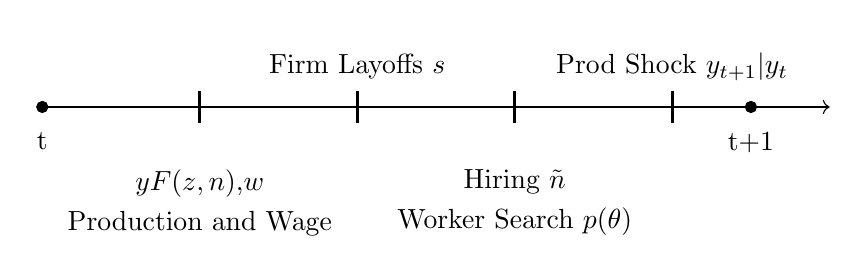
\begin{tikzpicture}[node distance=2mm]
  \draw[->] (0,0) to  (10,0);
    \filldraw[black] (0,0) circle (2pt);
  \node[below, black] at (0,-2mm) {t};
    \filldraw[black] (9,0) circle (2pt);
  \node[below, black] at (9,-2mm) {t+1};
  \foreach \x/\q in {2/,4/,6/,8/}{
    \draw[line width=1pt, black] (\x,-2mm) node[below, black](a\x){\q} -- (\x,2mm);
}
\node [below=of a2, align=center, minimum width=1in, minimum height=1cm] {$yF(z,n)$,$w$ \\ Production and Wage };
\node [above=of a4, align=center, minimum width=1in, minimum height=1cm] {Firm Layoffs $s$};
\node [below=of a6, align=center, minimum width=1in, minimum height=1cm] {Hiring $\tilde{n}$ \\ Worker Search $p(\theta)$};
\node [above=of a8, align=center, minimum width=1in, minimum height=1cm] {Prod Shock $y_{t+1}|y_t$};
\end{tikzpicture}
\caption{Within-period time line} \label{fig:Timing}
\end{figure}

Each period is divided into 4 stages, as illustrated in Figure~\ref{fig:Timing}. First, production takes place. Firm collects the output and pays wage $w$ to each worker it employs. Next, each firm lays off a fraction $s\geq 0$ of its workforce. Fired workers become unemployed, but may not search until the next period. The remaining workers, both employed and unemployed, then search for a job. This coincides with all the firm hiring $\tilde{n}$, from both entering and incumbent firms. All the hiring and search choices happen before the next productivity $y_{t+1}$ realizes and thus the agents have to rely on the expectation operator $E_{y_{t+1}|y_t}$.
%\subsubsection*{Physical Environment}
\subsubsection*{Information Structure and Contracts}
Upon hiring a worker, the firm commits to deliver expected utility $v$ via a contract. A contract defines the wage and
actions for a matched worker and firm for all future firm productivity histories $y^\tau\equiv (y_1,...,y_\tau)\mathcal{Y}^{\tau}$. The future history of firm productivity is common knowledge to both agents and is thus fully contractible. However, the match-specific productivity $z_{ij}$ is private information of the firm and worker's search decision $\hat{v}$ is private information of the worker. The contract $\mathcal{C}$ is then represented by 
\begin{equation}
\mathcal{C}=\{w_{\tau},s_{\tau},\hat{v}_\tau\}_{\tau=t}^\infty
\end{equation}
The first components captures firm's wage policy $w$ for each future productivity history. The second component captures \textit{expected} layoff probability $s$, given that the worker does not know the quality of their match. Note that these probabilities are not ex-ante: in histories where worker's information about their match quality updates, it will be reflected in all the corresponding layoff probabilities. An example of that could be a history where firm has faced multiple negative productivity shocks and was forced to lay off a vast majority of its workforce. The remaining workers will bayesian update that their match quality is now more likely to be high, and any future layoff probabilities will reflect that. 
The last component is worker's search decision. Although this action is unobserved by the firm, I focus on contracts where the contractual recommendations are incentive-compatible. The firm thus chooses workers’ search decisions, subject to the incentive compatibility constraint that the decisions match the workers’ optimal response.

%Add here a short discussion paragraph maybe???
The contract space is completely flexible in how wages and layoffs respond to productivity histories. In a setting with a continuum of contracts at the same time, this allows the firm to choose how to treat its heterogeneous (in quality and contracts) workforce: when a negative shock hits, who to fire and for whom to cut wages. This property is central to the paper and unique to the setting: unlike model with CRS production functions, these decisions depend on the state of the entire firm. Unlike other models of firm dynamics, with Nash Bargaining (\textcite{mccrary2022}) or Sequential Bargaining (\textcite{bilal2022}), the workers in the same firm may end up with different wages, layoffs, and their responses to productivity shocks. %By taking the model to the data, I am able to quantify how different firms, depending on their size and productivity, discriminate between their junior and senior workers.
\subsection{Value functions}
The above contract, and thus the problems of all the agents, can be described recursively. I start with the individual workers' problem and move on to firms managing contracts with a continuum of workers. I show that the state-space of the firm problem is discrete and, under a relatively weak approximation, bounded.
\subsubsection*{Worker's Problem} %Value functions, including search trade-off
Unemployed workers consume home production $b$. Each period, they search on the submarket that offers the best tradeoff between promised future utility and job finding probability. Dropping all time subscripts and focusing on a stationary equilibrium, the value of being unemployed $U$ can be written as:
\begin{equation} \label{unempproblem}
    U =\max_{v} u(b) + \beta[(1 - p(\theta_v))U + p(\theta_v)v]
\end{equation}

Consider an employed worker with an owed value $v$. Suppose a firm pays wage $w$ this period, will fire with probability $s$ and offers a lifetime expected utility $v'$ from tomorrow into the future. Then a worker faces the following search problem:
\begin{equation} \label{empproblem}
  v=\max_{\hat{v}} u(w) + \beta[sU + (1-s)[(1-p(\theta_{\hat{v}}))v'+p(\theta_{\hat{v}})\hat{v}]]   
\end{equation}
The optimal worker policy $\hat{v}$ depends only on the future offered utility $v'$. By raising $v'$, firm incentivizes its worker to search in higher $\hat{v}$, thus lowering the probability that the worker will leave.
Note that this can be equivalently rewritten as 
\begin{equation*}
  v=u(w) + \beta[sU + (1-s)R(v')]  
\end{equation*}
where $R(v') \equiv \max_{\hat{v}}[(1-p(\theta_{\hat{v}}))v'+p(\theta_{\hat{v}})\hat{v}]$ the optimal future value the worker gets upon being promised $v'$ and not being laid off.
\subsubsection*{Firm's Problem}
For now, consider the version of the model with no match heterogeneity ($z_0=0$ or $1$). A firm employs a measure $n$ of workers. Denote the distribution of their promised values $v$ that the firm owes to its workers as $P(v)$. Then for each of these values $v$, the firm has to choose the wage to pay $w_v$, the layoff rate $s_v$, and tomorrow, future productivity state-contingent promised value $v'_{v,y'}$. Firm may also hire $\tilde{n}$ workers at the value $\tilde{v}$.
The firm's problem can then be formulated recursively as follows:
\begin{equation*}
    \begin{split}
    J(y,n,P(v)) = & \max_{\tilde{n},\tilde{v},\{w_v,s_v,v'_{v,y'}\}} yF(n,z_0) - \int_v w_i dP(v_i) -\tilde{n}\frac{c}{q(\tilde{v})} -\kappa_f+ \beta E_{y'|y} J(y',n',P'(v)) \\
     s.t. \: & u(w_v) + \beta [s_v U + (1-s_v)R(v'_{v})=v] \; \forall v \\
    & v'_v = E_{y'|y} v'_{v,y'} \; \forall v \\
    & n' = n\int_v (1-s_v)(1-p(v'_v))dP(v)+\tilde{n} \\
    & n'P'(v) = n\int_v E_{y'|y}\mathbbm{1}_{v'_{v,y'}\leq v} (1-s_v)(1-p(v'_v))dP(v)+\mathbbm{1}_{\tilde{v}\leq v}\tilde{n}
    \end{split}
\end{equation*}
Firm has to maximize its net present value of profits subject to fulfilling every worker's promised value. 
Note that because the search decision happens before the next productivity state realizes, workers only care about the expected average promised value $v'_v$ when making their decisions rather than about any of the $v'_{v,y'}$ in particular. The latter two conditions specify the law of motion for firm size and the distribution of promised values. \\
\textbf{Discretizing the Problem} \label{subsection:discrete} In the current formulation, this problem is intractable as it involves a probability distribution, an uncountably infinitely-dimensional object, in the state-space. I first show that this state space can be discretized, thus bringing it ``down" to countably infinite states. Then I argue that restricting the state space to a finite number is \\
First, note that, when hiring, a firm chooses just one value at which to hire, $\tilde{v}$. This is an outcome of the directed structure of the labor market. Since a firm optimally decides in which submarket $v$ to post vacancies in \footnote{Assume no mixed strategies: in case a firm happens to be indifferent across multiple submarkets, it will only post vacancies in one of them.}, it will only hire from that submarket and thus at that value. This means that all the workers hired at the same time by the same firm are going to be at the same value, both at the time of hiring and in all the future periods. Therefore, it is equivalent to work with the cdf $P(v)$ or with the related probability mass function $\mathbb{P}(V=v)$: $P(v)=\sum_{v'\leq v}\mathbb{P}(V=v')$. 
Furthermore, for a firm of age $K<\infty$, there is at most $K$ different values $v$ such that $\mathbb{P}(V=v)>0$. These values correspond to the values owed to workers hired at different time periods, thus of different tenure at the firm $k=t-t_{hired}\leq K$.  One can then redefine the state space using tenure: 
\begin{lemma} \label{lemma_tenure}
A decision problem $J(y,n,P(v))$ of a firm of age $K$ can be equivalently represented as
\begin{equation*}
    \begin{split}
 J(y,\{n_k,v_k\}_{k\leq K}) =
    %Max
    & \max_{\tilde{n},\tilde{v},\{v'_{y',k},w_{k},s_{k}\}_{k\leq K}} 
    %Production
    yF(\sum_k n_k,z_0)-
    %Wage
    \sum_k w_kn_k \\
    %Size
    & -\tilde{n}\frac{c}{q(\tilde{v})}-\kappa_f
    %Expectation
    +\beta E_{y'|y} J(y',\{n'_k,v'_{y',k}\}_{k\leq K+1}) \\
     s.t. \: & u(w_k) + \beta [s_k U + (1-s_k)R(v'_{k+1})=v_k] \; \forall k\leq K \\
    & v'_{k+1} = E_{y'|y} v'_{y',k+1} \; \forall k\leq K \\
    & n'_{k+1} = n_k(1-s_k)(1-p(v'_{k+1}))+\tilde{n}\; \forall k\leq K \\
    & n'_0 = \tilde{n}, v'_0 = \tilde{v}
    \end{split}
\end{equation*}
\end{lemma}
\textbf{Contracts Converge}
This tenure-based formulation of the problem allows me to work with a discrete, although expanding, state-space. Finally, to make this fully tractable, I note that wages in contracts tend to converge, suggesting that $v_k\approx v_{k+1} \forall k\geq\bar{k}$. I derive this result in the following propositions. The idea follows a theoretical result from \textcite{balke2022}'s Proposition 3 that wages in dynamic contracts tend to always follow a ``target wage". I adapt their result to my model with a continuum of contracts.
\newline
%I adapt the Proposition 3 from \textcite{balke2022}, which establishes that wages in each match track a "target wage", to my model with a continuum of contracts. 
To show that the wages converge, I start by characterizing the wage growth.
\begin{proposition} \label{prop:wagegrowth}
  For any current state $(y,\{n_k,v_k,z_k\})$, wages change according to the following relationship:
\begin{equation} 
    \frac{1}{u'(w'_{k+1})} - \frac{1}{u'(w_k)} = \eta(v'_{k+1}) E_{y'|y} \frac{\partial J(y',\{n'_k,v'_{y',k}\})}{\partial n'_{k+1}}
\end{equation}
where $\eta(v'_{k+1}) = \frac{\partial log(1-p(v'))}{\partial v'}$ is the semi-elasticity of the job-finding probability with respect to the promised value $v'_{k+1}$.
\end{proposition}
\begin{proof}
  See Appendix \ref{proof:wagegrowth}.
\end{proof}
The relationship is at the core of the firm's insurance vs incentive provision trade-off: while the marginal value of the worker $\frac{\partial J(y',\{n'_k,v'_k,z'_k\})}{\partial n'_{k+1}}$ is positive, the firm is intent on keeping its workers, and thus chooses to backload wages, thus incentivizing the workers to stay at the cost of higher total wage payments. On the flip side, if the marginal worker value is negative, the firm will choose to lower wages, incentivizing workers to leave. This brings us to the result on contract convergence:
\begin{proposition} \label{prop:targetwage}
 Fix firm's state $(y,\{n_k,v_k\})\equiv (y,n,P(v))$ and define $v^*$ such that \\ 
 $E_{y'|y}\frac{\partial J(y',n',P(v'))}{\partial P(v^*)}=0$. Then
  \[ |w'_{k+1}-w^*_{v^*}|<|w_k-w^*_{v^*}| \; \forall k\]
 Moreover, defining $\bar{k}\equiv arg\max_k v_k$,
 \[ w'_{\bar{k}+1}-w'_{k+1}<w_{\bar{k}}-w_k \; \forall k\neq\bar{K}\]
 
%Consider workers at tenure step $k$. Their wages will rise as long as $\frac{\partial J(y',\{n'_k,v'_k,z'_k\})}{\partial n'_{k+1}}>0$ and until $\frac{\partial J(y',\{n'_k,v'_k,z'_k\})}{\partial n'_{k+1}}=0$. Absent quality heterogeneity ($z_0=0$ or $z_0=1$), 
%\[\forall k: $w_k \rightarrow w^*_y$\]
%Where \frac{}
\end{proposition}
\begin{proof}
  See Appendix~\ref{proof:targetwage}
\end{proof}
This proposition suggests that, across all tenure steps, wages change in the direction of the target wage $w^*_{v^*}$. Moreover, they do so in a way that contracts the incumbent wage space, lowering the difference between the highest and all other wages. Then, for workers that have been at the firm for long enough, this process of constant movement towards the target wage will result in convergence of wages. \\
Empirically, I show in Appendix \ref{wagegrowthK} that wage growth in France stagnates after about 10 years of tenure.  This allows me to restrict attention to finite and constant $K$ for all the firms in my quantitative exploration. Note that this is only an approximation since, as $K\rightarrow\infty$, the model approaches the problem described in Lemma \ref{lemma_tenure}.
\newline
\textbf{Introducing Heterogeneity}  I stick to the theoretical formulation in Lemma \ref{lemma_tenure} and introduce heterogeneity in match quality. With $0<z_0<1$, matches employed by the firm may be of both high and low quality. I do not allow the firm to choose quality-contingent wages, thus the firm can only influence match quality via layoffs \footnote{I show in Appendix \ref{microfoundation} that, under a sufficiently low elasticity of on-the-job search, this is in fact an outcome of the firm's optimal information allocation problem.}. \\
Although any particular worker does not know their own match quality, they know the proportion of high quality matches in their cohort. All new hires start with a proportion $z_0$ of high matches, and, although it may evolve, all the workers of the same tenure $k$ will have the same probability of having a high quality match $z_k\geq z_0$. This probability is common knowledge to the firm and all its workers and depends on layoffs in the corresponding cohort to $z'_{k+1}=min(\frac{z_k}{1-s_k},1)\; \forall k\leq K$.
\\
\begin{definition} \label{firmproblem}
The complete firm decision problem involves
\begin{equation*}
    \begin{split}
 J(y,\{n_k,v_k,z_k\}_{k\leq K}) =
    %Max
    & \max_{\tilde{n},\tilde{v},\{v'_{y',k},w_{k},s_{k}\}_{k\leq K}} 
    %Production
    yF(\sum_k n_k,\frac{\sum n_kz_k}{\sum n_k})-
    %Wage
    \sum_k w_kn_k \\
    %Size
    &-\tilde{n}\frac{c}{q(\tilde{v})}-\kappa_f
    %Expectation
    +\beta E_{y'|y} J(y',\{n'_k,v'_k,z'_k\}_{k\leq K+1}) \\
     s.t. \: & u(w_k) + \beta [s_k U + (1-s_k)R(v'_{k+1})=v_k] \; \forall k\leq K \\
    & v'_{k+1} = E_{y'|y} v'_{k+1,y'} \; \forall k\leq K \\
    & n'_{k+1} = n_k(1-s_k)(1-p(v'_{k+1}))+\tilde{n}\; \forall k\leq K \\
    & z'_{k+1} = min(\frac{z_k}{1-s_k},1)\; \forall k\leq K \\
    & n'_0 = \tilde{n}, v'_0 = \tilde{v}, z'_0 = z_0
    \end{split}
\end{equation*}
\end{definition}


\subsubsection*{Free-entry and exit}
Firms are free to enter the market and start producing upon paying an entry cost $\kappa_e$. Upon entry, firms draw a productivity shock and start with a single worker. Thus, the free-entry condition pins down the expected profits of firms upon entry:
\begin{equation} \label{freeentry}
    \kappa_e\geq \max_{v_0} -\frac{c}{q_{v_0}}+\beta E_y J(y,\{1,0,...\},\{v_0,...\},\{z_0,...\})
\end{equation}
When taking the model to the data, this results in a negative connection between the cost of entry $\kappa_e$ and the probability to fill a vacancy $q(\theta)$: the cheaper it is to enter, the tighter will the labor market be, thus making it easier for workers to find jobs and harder for firms to fill vacancies.
\\
Similarly to new firms, incumbent firms have to pay an operating cost $\kappa_f$ every period to stay open. With $\kappa_f$ already included into the firm value function, firms stay open if 
\begin{equation} \label{freeexit}
    J(y,\{n_k\},\{v_k\},\{z_k\})\geq 0
\end{equation}

\subsection{Equilibrium}
A complete equilibrium is a set of value functions, policies, matching rates, and distribution of workers and firms for each labor market $v$ such that 
\begin{itemize}
    \item Firms solve the problem from Definition \ref{firmproblem}
    \item Workers solve search problems from Equations \ref{unempproblem} and \ref{empproblem}
    \item Free-entry  and free exit conditions \ref{freeentry},\ref{freeexit}  are satisfied
    \item Job-finding and vacancy-filling probabilities are consistent with the matching function
    \item Tightness function $\theta_v$ is consistent with the firm posting and worker search strategies
    \item Labor market clears
\end{itemize}
Under an additional assumption in Appendix \ref{blocrecur}, I show that the equilibrium may be block recursive, meaning independent of the distribution of workers and firms. I use that assumption in the quantitative exploration, but not in the theoretical discussion, where instead I focus my attention on the steady-state of the economy described above.

\subsection{Mechanism}
I now show how the model delivers the heterogeneity in wage and layoff passthrough across tenure. 
I first characterize the FOC for layoffs:
\begin{proposition} \label{prop:layoffs}
  Fix a firm state $(y,\{n_k,v_k,z_k\})$. Layoffs are characterized by the following first-order condition:
  \begin{equation}
    -E_{y'|y}\frac{\partial J'}{\partial n'_{k+1}}(1-p(v'_{k+1}))+E_{y'|y}\frac{\partial J'}{\partial z'_{k+1}}\frac{\partial z'_{k+1}}{\partial s_k}\frac{1}{n_k} - \frac{R(v'_{k+1})-U}{u'(w_k)}\leq 0
  \end{equation}
  and $s_k \geq 0$ with complementary slackness.
\end{proposition}
\begin{proof}
  See Appendix \ref{proof:layoffs}
\end{proof}
Just like wages, the trade-off for layoffs primarily revolves around the value of the marginal worker $E_{y'|y}\frac{\partial J'}{\partial n'_{k+1}}$ and the cost of having to compensate the worker $\frac{R(v'_{k+1})-U}{u'(w_k)}$. The truly unique component to layoffs is the quality effect $E_{y'|y}\frac{\partial J'}{\partial z'_{k+1}}\frac{\partial z'_{k+1}}{\partial s_k}\frac{1}{n_k}$. \\
Though not obvious from this condition, workers on higher values are less likely to be laid off: even absent heterogeneity in quality, the cost of firing rises faster in promised value than the value of the marginal worker falls. \\
I now connect the layoffs and wage cuts:
\begin{proposition} \label{prop:wage_cuts}
Let $K_s\equiv \{k\leq K|s_k>0\}$. In states where $K_s$ is non-empty:
  \[w'_{k+1}-w_k>w'_{k'+1}-w_{k'} \: \forall k\in K_s,k'\notin K_s\]
\end{proposition}
\begin{proof}
 Start with the wage growth equation from Proposition \ref{prop:wagegrowth}, extended to the case of heterogeneous matches. 
     \[\frac{1}{u'(w'_{k+1})} - \frac{1}{u'(w_k)} = \eta(v'_{k+1}) E_{y'|y} \frac{\partial J(y',\{n'_k,v'_{y',k},z'_k\})}{\partial n'_{k+1}}\]
     One can now apply the Envelope Theorem to extend the RHS of the equation:
     \begin{align*}
     E_{y'|y} \frac{\partial J(y',\{n'_k,v'_{y',k},z'_k\})}{\partial n'_{k+1}}  = & E_{y'|y}\Big[y'\frac{\partial F(\sum n'_k,\frac{\sum n'_k z'_k}{\sum n'_k})}{\partial n'_{k+1}} - w'_{k+1} + \\
     & \beta (1-p(v''_{k+2}))(1-s'_{k+1})E_{y''|y'} \frac{\partial J(y'',\{n''_k,v''_{y'',k},z''_k\})}{\partial n''_{k+2}})\Big]      
     \end{align*}
     One can note that the production derivative $\frac{\partial F(\sum n'_k,\frac{\sum n'_k z'_k}{\sum n'_k})}{\partial n'_{k+1}}$ is increasing in $z'_{k+1}$. And, moreover, that $\frac{\partial^2 F(\sum n'_k,\frac{\sum n'_k z'_k}{\sum n'_k})}{\partial n'_{k+1} \partial z'_{k+1}}> \frac{\partial^2 F(\sum n'_k,\frac{\sum n'_k z'_k}{\sum n'_k})}{\partial n'_{k'} \partial z'_{k+1}}, k'\neq k+1$. This implies that, the workers in steps $k \in K_s$ will experience the largest rise in marginal productivity. \textcolor{red}{This doesn't mean that they are at the highest marginal productivity though! Part of my intuition is predicated on the fact that the other workers, ones not fired, are already quite close to their target wages! Otherwise those guys would still have the best wage growth. Essentially, my intuition is that the fired cohorts receive a spike in marginal productivity, so, if they're on the similar-ish wage path to the other cohorts, they should get the best wage growth. But this needs to be formalized some more.}
\end{proof}
The intuition behind this result is that layoffs give a second-order push-up effect on wages: since the remaining workers are now of higher quality, there is less incentive to cut those workers' wages. And, although higher tenure steps may be of even higher quality, because their quality effect has already had to be internalized in wages, their wage cuts will in fact be larger than the cuts of just recently fired workers.
%\input{quantitative}




%%%%%%%%%%%%%%%%%%%%%%%%%%%%%%%%%%%%%%%

\section{Conclusion}
%I estimate wage cyclicality separately for different jobs, based on their hiring pools. I use the matched employer-employee data to find that wages, both for new and incumbent workers, are significantly more rigid in jobs hiring from unemployment than in jobs poaching workers. I then simulate a model incorporating the separation of search and heterogeneous wage rigidity across different submarkets to find that wage rigidity in the entry-level submarket matters significantly more for the volatility of unemployment than in the higher submarkets. Together, the empirical and the theoretical results imply that, for unemployment volatility purposes, wages are highly rigid. I confirm this by comparing the heterogeneous wage cyclicality calibration of the model to the homogeneous one and find that accounting for the heterogeneity across jobs increases the unemployment volatility by $20\%$.
%Moreover, the higher up the ladder is the submarket, the less important is its wage rigidity.  This goes in the direction of solving the unemployment volatility puzzle.

%Potential interesting application of the empirical result could be explaining some of the business cycle-related job ladder facts. As one example, \textcite{moscarini2018} find that the job-to-job transition rate is procyclical, and especially so at the bottom of the job ladder. This might be because wages at the bottom of the ladder are too high during recessions, thus disincentivizing workers from transitioning to a different job. It would also be interesting to understand where the observed heterogeneity in wage cyclicality stems from. 
\newpage
\printbibliography %Prints bibliography



\appendix
\section{Model Appendix} 
\subsection{Proofs}
\subsubsection*{Proof of Proposition \ref{prop:wagegrowth}} \label{proof:wagegrowth}
\subsubsection*{Proof of Proposition \ref{prop:targetwage}} \label{proof:targetwage}
\subsubsection*{Proof of Proposition \ref{prop:layoffs}} \label{proof:layoffs}
\subsection{Tenure-specific Severance Payments} \label{severance}
I allow the firm to offer tenure-specific severance payments $sev_k$ to its workers. The severance is constant over time and paid perpetually upon firing and before finding a new job. I show that the severance structure involves higher payments for longer tenured workers (if those workers are on a higher promised value). 
\begin{proposition}
\label{severanceprop}
Fix a firm state. Its severance payments for each tenure $k$ are given by
\begin{equation*}
    \begin{split}
    & \frac{u'(b+sev_k)}{u'(w_k)}=1-\frac{\beta sev_k \frac{\partial p(\theta_{sev_k})}{\partial sev_k}}{1-\beta(1-p(\theta_{sev_k}))} \\
    & \theta_{sev_k} = \theta(arg \max_v [(1-p(v))U(sev_k)+p(v)v]) \\
    \end{split}
\end{equation*}
\end{proposition}
\begin{proof}
I start by describing the unemployment value of a worker with severance payment $sev_k$:
\[U(sev_k) = u(b+sev_k) + \beta \max_v[(1-p(\theta_v))U(sev_k)+p(\theta_v)v]\]
Denote the probability of finding a job with severance payment $sev_k$ as $p(\theta_{sev_k})$. The extra value to the unemployed from the severance payment is then given by
\[\frac{\partial U(sev_k)}{\partial sev_k} = u'(b+sev_k) + \beta (1-p(\theta_{sev_k}))U'(sev_k)=\frac{u'(b+sev_k)}{1-\beta(1-p(\theta_{sev_k}))}\]
Then the total benefit to the firm from raising the severance payment is the slackening of the promised-keeping constraint thanks to this rise in the unemployment value:
\[\lambda_k n_k \beta s_k \frac{\partial U(sev_k)}{\partial sev_k} = \frac{n_k}{u'(w_k)}\beta s_k \frac{u'(b+sev_k)}{1-\beta(1-p(\theta_{sev_k}))}\]
On the cost side, the firm internalizes the net present value of the severance payments when firing $n_ks_k$ workers:
\[\frac{\partial}{\partial sev_k}\Big[n_k s_k \beta \frac{sev_k}{1-\beta(1-p(\theta_{sev_k}))}\Big]=n_ks_k\beta \frac{[1-\beta(1-p(\theta_{sev_k}))]-\beta sev_k \frac{\partial p(\theta_{sev_k})}{\partial sev_k}}{[1-\beta(1-p(\theta_{sev_k}))]^2}\]
The optimal severance payment then follows from the first-order condition:
\[ \frac{n_k}{u'(w_k)}\beta s_k \frac{u'(b+sev_k)}{1-\beta(1-p(\theta_{sev_k}))} = n_ks_k\beta \frac{[1-\beta(1-p(\theta_{sev_k}))]-\beta sev_k \frac{\partial p(\theta_{sev_k})}{\partial sev_k}}{[1-\beta(1-p(\theta_{sev_k}))]^2}\]
Rearranging gives the result.
\[\frac{u'(b+sev_k)}{u'(w_k)}=1-\frac{\beta sev_k \frac{\partial p(\theta_{sev_k})}{\partial sev_k}}{1-\beta(1-p(\theta_{sev_k}))}\]
\end{proof}
Note that, besides $u'(w_k)$, all the components of the severance payment are independent of both the firm state and the worker tenure. 
It is immediate to notice then that higher paid workers will have higher severance payments: as $\frac{1}{u'(w_k)}$, the value to the firm of the severance payment goes up, while costs stay the same. Therefore, the firm will optimally choose to offer higher severance payments to higher paid workers. \\
This equation is also easy to implement numerically: using the formulation in Appendix~\ref{dual}, where $\rho_k\equiv u'(w_k)$ is a state variable, I can immediately compute the payments for all the firm states, before solving the rest of the firm problem.
\subsection{Microfounding the Wage Noncontractability} \label{microfoundation}
Consider a simplified, 2-period version of the model. The firm starts with measure $n=2$ of workers, half of them of high quality and the other half of low. I allow the firm to offer quality-contingent wages in whichever way it likes. \\
I show that, under a sufficiently small elasticity of job search probability with respect to promised value $v'$, $\eta(v')\equiv\frac{\partial (1-p(v')) /\partial v'}{(1-p(v'))}$, the firm will optimally choose to keep wages constant across matches of different quality.
\subsection{Recursive Lagrangian Approach} \label{dual}
The original design of the problem would require solving promised values $v'_{y',k}$ for both each tenure step and each future productivity state. Following \textcite{balke2022}, I solve the following Pareto problem:
\begin{equation*}
\begin{split}
\mathcal{P}(y,\{n_k,\rho_k,z_k\}) = &\inf_{\omega_k} \sup_{\tilde{n},\tilde{v},\{w_k,s_k,v'_k\}}  yF(n,z) - \sum_k n_kw_k - \kappa_f - \tilde{n}\frac{c}{q(\theta_{\tilde{v}})}   \\
& + \sum_k\rho_k(u(w_k)+\beta[s_kU+(1-s_k)R(v'_{k+1})] \\
& -\beta\sum_k \omega_k v'_{k+1}+\beta E_{y'|y}\mathcal{P}(y',\{n'_k,\omega_k,z'_k\})    
\end{split}
\end{equation*}

where
\[\mathcal{P}(y,\{n_k,\rho_k,z_k\}) \equiv \sup_{\{v_k\}} J(y,\{n_k,v_k,z_k\})+\sum_k \rho_k v_k \]
The following proof (for $K\rightarrow\infty$ but the proof extends trivially to finite $K$) establishes its equivalence with the initial problem. It follows the steps of \textcite{balke2022}, extending it to the case of a multi-worker firm.
\begin{proof}
We have the following recursive formulation for $J$:
\begin{equation*}
    \begin{split}
 J(y,\{n_k,v_k,z_k\}_{k\leq K}) =
    %Max
    & \max_{\tilde{n},\tilde{v},\{v'_k,v'_{y',k},w_{k},s_{k}\}_{k\leq K}} 
    %Production
    yF(\sum_k n_k,\frac{\sum n_kz_k}{\sum n_k})-
    %Wage
    \sum_k w_kn_k
    %Size
    -\tilde{n}\frac{c}{q(\tilde{v})}-\kappa_f \\
    %Expectation
    & +\beta E_{y'|y} J(y',\{n'_k,v'_k,z'_k\}_{k\leq K+1}) \\
(\lambda_k) \: & u(w_k) + \beta [s_k U + (1-s_k)R(v'_{k+1})=v_k] \; \forall k\leq K \\
(\omega_k)    & v'_{k+1} = E_{y'|y} v'_{k+1,y'} \; \forall k\leq K \\
    & n'_{k+1} = n_k(1-s_k)(1-p(v'_{k+1}))+\tilde{n}\; \forall k\leq K \\
    & z'_{k+1} = min(\frac{z_k}{1-s_k},1)\; \forall k\leq K \\
    & n'_0 = \tilde{n}, v'_0 = \tilde{v}, z'_0 = z_0
    \end{split}
\end{equation*}
Consider the Pareto problem
\[\mathcal{P}(y,\{n_k,\rho_k,z_k\}) = \sup_{\{v_k\}} J(y,\{n_k,v_k,z_k\})+\sum_k \rho_k v_k \]
I first substitute the definition of $J$ together with its constraints into $\mathcal{P}$:
\begin{equation*}
    \begin{split}
 \mathcal{P}(y,\{n_k,\rho_k,z_k\}) =
    %Max
    & \sup_{\tilde{n},\tilde{v},\{v_k,v'_{k},v'_{y',k},w_{k},s_{k}\}_{k\leq K}} 
    %Production
    yF(\sum_k n_k,\frac{\sum n_kz_k}{\sum n_k})-
    %Wage
    \sum_k w_kn_k
    %Size
    -\tilde{n}\frac{c}{q(\tilde{v})}-\kappa_f \\
    %Expectation
    & +\beta E_{y'|y} J(y',\{n'_k,v'_k,z'_k\}_{k\leq K+1}) + \sum_k \rho_k v_k  \\
(\lambda_k) \: & u(w_k) + \beta [s_k U + (1-s_k)R(v'_{k+1})=v_k] \; \forall k\leq K \\
(\omega_k) \:   & v'_{k+1} = E_{y'|y} v'_{k+1,y'} \; \forall k\leq K \\
    & n'_{k+1} = n_k(1-s_k)(1-p(v'_{k+1}))+\tilde{n}\; \forall k\leq K \\
    & z'_{k+1} = min(\frac{z_k}{1-s_k},1)\; \forall k\leq K \\
    & n'_0 = \tilde{n}, v'_0 = \tilde{v}, z'_0 = z_0
    \end{split}
\end{equation*}
I now substitute in the promise-keeping constraint:
\begin{equation*}
    \begin{split}
 \mathcal{P}(y,\{n_k,\rho_k,z_k\}) =
    %Max
    & \sup_{\tilde{n},\tilde{v},\{v'_k,v'_{y',k},w_{k},s_{k}\}_{k\leq K}} 
    %Production
    yF(\sum_k n_k,\frac{\sum n_kz_k}{\sum n_k})-
    %Wage
    \sum_k w_kn_k
    %Size
    -\tilde{n}\frac{c}{q(\tilde{v})}-\kappa_f \\
    %Expectation
    & +\beta E_{y'|y} J(y',\{n'_k,v'_k,z'_k\}_{k\leq K+1}) + \sum_k \rho_k (u(w_k) + \beta [s_k U + (1-s_k)R(v'_{k+1})])  \\
(\omega_k) \:    & v'_{k+1} = E_{y'|y} v'_{k+1,y'} \; \forall k\leq K \\
    & n'_{k+1} = n_k(1-s_k)(1-p(v'_{k+1}))+\tilde{n}\; \forall k\leq K \\
    & z'_{k+1} = min(\frac{z_k}{1-s_k},1)\; \forall k\leq K \\
    & n'_0 = \tilde{n}, v'_0 = \tilde{v}, z'_0 = z_0
    \end{split}
\end{equation*}
I introduce the $\omega_k$-constraints with weights $\beta$ into the problem:
\begin{equation*}
    \begin{split}
 \mathcal{P}(y,\{n_k,\rho_k,z_k\}) =
    %Max
    & \inf_{\{\omega_k\}}\sup_{\tilde{n},\tilde{v},\{v'_k,v'_{y',k},w_{k},s_{k}\}_{k\leq K}} 
    %Production
    yF(\sum_k n_k,\frac{\sum n_kz_k}{\sum n_k})-
    %Wage
    \sum_k w_kn_k
    %Size
    -\tilde{n}\frac{c}{q(\tilde{v})}-\kappa_f \\
    %Expectation
    & +\beta E_{y'|y} J(y',\{n'_k,v'_k,z'_k\}_{k\leq K+1}) + \sum_k \rho_k (u(w_k) + \beta [s_k U + (1-s_k)R(v'_{k+1})])  \\
    & + \sum_k \beta\omega_k(E_{y'|y}v'_{y',k+1}-v'_{k+1})\\
    & n'_{k+1} = n_k(1-s_k)(1-p(v'_{k+1}))+\tilde{n}\; \forall k\leq K \\
    & z'_{k+1} = min(\frac{z_k}{1-s_k},1)\; \forall k\leq K \\
    & n'_0 = \tilde{n}, v'_0 = \tilde{v}, z'_0 = z_0
    \end{split}
\end{equation*}
I then rearrange the value function by moving $E_{y'|y}\sum_k \beta\omega_kn'_{k+1}v'_{y',k+1}$ (additional constraints are dropped to simplify notation):
\begin{equation*}
    \begin{split}
 \mathcal{P}(y,\{n_k,\rho_k,z_k\}) =
    %Max
    & \inf_{\{\omega_k\}}\sup_{\tilde{n},\tilde{v},\{v_k,v'_{y',k},w_{k},s_{k}\}_{k\leq K}} 
    %Production
    yF(\sum_k n_k,\frac{\sum n_kz_k}{\sum n_k})-
    %Wage
    \sum_k w_kn_k
    %Size
    -\tilde{n}\frac{c}{q(\tilde{v})}-\kappa_f \\
    %Expectation
    & +\beta E_{y'|y} [J(y',\{n'_k,v'_k,z'_k\}_{k\leq K+1}) + \sum_k\omega_kv'_{y',k+1}]\\
    & \sum_k \rho_k (u(w_k) + \beta [s_k U + (1-s_k)R(v'_{k+1})])- \sum_k \beta\omega_kv'_{k+1}  
    \end{split}
\end{equation*}
Lastly, I split the sup:
\begin{equation*}
    \begin{split}
    \mathcal{P}(y,\{n_k,\rho_k,z_k\}) =
    %Max
    & \inf_{\{\omega_k\}}\sup_{\tilde{n},\tilde{v},\{v'_k,w_{k},s_{k}\}_{k\leq K}} 
    %Production
    yF(\sum_k n_k,\frac{\sum n_kz_k}{\sum n_k})-
    %Wage
    \sum_k w_kn_k
    %Size
    -\tilde{n}\frac{c}{q(\tilde{v})}-\kappa_f \\
    %Expectation
    & +\beta E_{y'|y} [\sup_{v'_{y',k+1}}J(y',\{n'_k,v'_k,z'_k\}_{k\leq K+1}) + \sum_k\omega_kv'_{y',k+1}]\\
    & \sum_k \rho_k (u(w_k) + \beta [s_k U + (1-s_k)R(v'_{k+1})])- \sum_k \beta\omega_kv'_{k+1}     
    \end{split}
\end{equation*}
From this, one can note that, by definition of $\mathcal{P}$ \[\sup_{v'_{y',k+1}}J(y',\{n'_k,v'_k,z'_k\}_{k\leq K+1}) + \sum_k\omega_kv'_{y',k+1} = \mathcal{P}(y',\{n'_k,\omega_k,z'_k\})\]
We thus arrive to the formulationof the problem as described at the beginning, not involving finding future state-specific promised values $v'_{y',k}$.
\end{proof}
\subsection{Block Recursivity} \label{blocrecur}
I introduce an assumption that would allow for a block recursive eqiulibrium under the same conditions as in \textcite{schaal2017}. Block recursivity requires an indifference condition, either on the side of the firms or on the side of the workers. Under two-sided ex-post heterogeneity, that is not immediately achievable. \\
\textcite{schaal2017} shows that, in a setting similar to mine, but with transferable utility between workers and firms, which he achieves due to the risk-neutral worker utility function, firms all have the same preferences across all the submarkets that they may post vacancies in. 
Define the minimal hiring cost as 
\[k = \min_{v} [v + \frac{c}{q_v}]\]
Due to transferable utility, the cost of employing the worker from submarket $v$ becomes simply the value $v$. Thus, the optimal entry of vacancies in \textcite{schaal2017} can be summarized by 
\[\theta_v [v + \frac{c}{q_v} - k]=0\]
Meaning that either a submarket $v$ minimizes the hiring cost or it is closed. This condition is completely independent of the distribution of firms and workers, exactly because the one component where the firm type might come through, the cost of employing a worker from submarket $v$, is completely independent from the firm's state due to transferable utility.\\
Utility is not transferable in my model, and thus different firms may face different costs of employing a worker at some value $v$ (for example, fixing $y$ and $z$, small firms prefer high values $v$ due to their intention to upsize). To get around that, I split the value $v$ that the worker would get upon getting hired into two components, the sign-on wage $w_v$ and the remaining value $v_0$ such that
\[u(w_v)+\beta v_0= v\]
This additional wage payment is incurred immediately upon hiring, allowing the remaining value that the firm owes to its worker, $v_0$, to be completely independent of the submarket $v$. Essentially, from the firm's perspective, submarkets now differ not in the value that firms would owe to the workers, but in this sign-on wage. The cost minimization problem then becomes 
\[k = \min_{v} [w_v + \frac{c}{q_v}]\]
This problem is now again completely independent of the firm's state, and thus the distribution of firms and workers no longer affects the tightness function $q_v$.\textcite{schaal2017} shows that, in a setting similar to mine, but with transferable utility between workers and firms, which he achieves due to the risk-neutral worker utility function, firms all have the same preferences across all the submarkets that they may post vacancies in. Then setting $\theta_v$ such that 
\newpage
\section{Quantitative Appendix}
% Define colors
\definecolor{state}{RGB}{0,128,0}       % green
\definecolor{ctrl}{RGB}{255,140,0}      % orange
\definecolor{ex}{RGB}{255,0,255}        % magenta
\definecolor{nextstate}{RGB}{0,0,255}    % blue
\definecolor{value}{RGB}{128,128,0}    % yellow

\subsection{Variables}
\subsection*{\textcolor{state}{Endogenous state variables}}
\begin{align*}
&\textcolor{state}{\{n_{k}\}_{k\leq K}}, \textcolor{state}{\{\rho_{k}}, \textcolor{state}{z_{k}\}_{1\leq k\leq K}}
\end{align*}
\textbf{Code:} \texttt{states: size, rho, q}

\subsection*{\textcolor{ex}{Exogenous state variables}}
\begin{align*}
&\textcolor{ex}{y}
\end{align*}
\textbf{Code:} \texttt{z}

\subsection*{\textcolor{ctrl}{Control variables}}
\begin{align*}
&\textcolor{ctrl}{\tilde{n}}, \textcolor{ctrl}{\{\rho'_k\}_{1\leq k\leq K}}, \textcolor{ctrl}{\{s_k\}_{k\leq K}}
\end{align*}
\textbf{Code:} \texttt{hiring, rho\_star, sep\_star}

\subsection*{\textcolor{value}{Value function}}
\begin{align*}
&\textcolor{value}{\mathcal{P}(\textcolor{ex}y,\textcolor{state}{\{n_k,\rho_k,z_k\}})}
\end{align*}
\textbf{Code:} \texttt{ERho\_star, EJ\_star}
\subsection{Equations}
Equations (1)--(21): \textcolor{value}{Value function in olive} (given by value and its gradient guesses from future states), \textcolor{state}{states in }\textcolor{state}{green} (given), \textcolor{ctrl}{controls} in \textcolor{ctrl}{orange} (given by policy guess from current states), next period \textcolor{ex}{exogenous states in magenta} (to be summed over), next period \textcolor{nextstate}{states in blue}, parameters in black.
\begin{align}
%0&=\textcolor{ctrl}{\rho^*_{k+1}}-\textcolor{state}{\rho_k} - \eta(v'_{k+1})E\frac{\partial J(\textcolor{ex}{y'},\textcolor{nextstate}{\{n'_k,v'_{y',k},z'_k\})}}{\partial \textcolor{nextstate}{n'_{k+1}}} \\
0&=\textcolor{ctrl}{\rho'_{k+1}}-\textcolor{state}{\rho_k} - \eta(E \frac{\partial P(\textcolor{ex}{y'},\textcolor{nextstate}{\{n'_k,\rho'_{k},z'_k\})}}{\partial \textcolor{nextstate}{\rho'_{k+1}}})E\frac{\partial \mathcal{P}(\textcolor{ex}{y'},\textcolor{nextstate}{\{n'_k,\rho'_{k},z'_k\})}}{\partial \textcolor{nextstate}{n'_{k+1}}} \\
% ... (rest of equations unchanged for brevity) ...
\end{align}


\section{Data Appendix}
\
\subsection{Wage Growth} \label{wagegrowthK}
I use the same sample to plot the log (real) wage growth across first 30 years of tenure. 
\includegraphics[width=0.75\textwidth]{Wage growth across tenure under 30,cutoff 100.jpg} \\
The wage growth appears to flatten after about 10 years of tenure, suggesting that it is not quantitatively costly to use $K=10$ as an approximation of the firm problem from Definition \ref{firmproblem}.






\end{document}